\documentclass{article}
\usepackage[utf8]{inputenc}
\usepackage[english]{babel}
\usepackage{amsthm}
\usepackage{amssymb}
\usepackage{mathcomp}
\usepackage{amsmath}
\usepackage{natbib}
\usepackage{array}
\usepackage{wrapfig}
\usepackage{multirow}
\usepackage{tabularx}
\usepackage{multirow}
\usepackage{graphicx}

\newtheorem{ishaan}{Theorem}[section]
\newtheorem{lemma}{Lemma}[section]
\renewcommand\qedsymbol{$\blacksquare$}

\title{Homework 4}
\author{Sean Eva}
\date{September 2021}

\begin{document}

\maketitle

\begin{enumerate}
    \item 
    
    $log_{10}(\frac{0.067}{3302.98})=-4.693$\\
    $log_{10}(\frac{0.560}{5895.94})=-4.022$\\
    $log_{10}(\frac{fN_a\lambda}{5000\AA})=12.80$ for $\lambda=3302.98$\AA\\
    $log_{10}(\frac{fN_a\lambda}{5000\AA})=14.60$ for $\lambda=5895.94$\AA\\
    $log_{10}(\frac{(0.0049)(3302.98)}{5000})=-2.48$\\
    $log_{10}(\frac{(0.3250)(5895.94)}{5000})=-0.42$\\
    $12.80-(-2.48)=15.28$\\
    $14.6-(-0.42)=15.02$\\
    Then the average value of $log_{10}N_a$ is $15.15$. Therefore there are $10^{15.15}N_a$ per unit area of the sun's photosphere.\\
    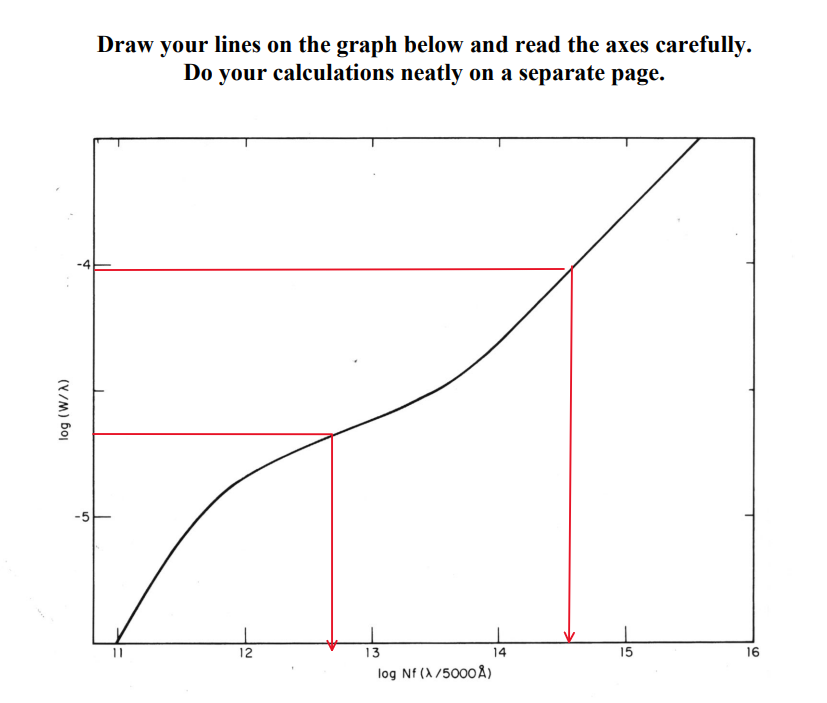
\includegraphics[width=0.75\textwidth]{Graph for HW3.png}
    
    \item
    
    $\Delta\lambda=\frac{\lambda}{c}\sqrt{\frac{2kT}{m}}$\\
    Atomic Mass of Calcium: $40.078*1.66*10^{-27}=66.53*10^{-27}$kg\\
    $T=3000\text{k}:$\\
    \begin{align*}
        \Delta\lambda &= \frac{393.3*10^{-9}}{3*10^8}\sqrt{\frac{2(1.38*10^{-23})(3000)}{66.53*10^{-27}}}\\
        &= 1.46*10^{-3}\text{nm}
    \end{align*}
    $T=6000\text{k}:$\\
    \begin{align*}
        \Delta\lambda &= \frac{393.3*10^{-9}}{3*10^8}\sqrt{\frac{2(1.38*10^{-23})(6000)}{66.53*10^{-27}}}\\
        &= 2.06*10^{-3}\text{nm}
    \end{align*}
    $T=12000\text{k}:$
    \begin{align*}
        \Delta\lambda &= \frac{393.3*10^{-9}}{3*10^8}\sqrt{\frac{2(1.38*10^{-23})(12000)}{66.53*10^{-27}}}\\
        &= 2.92*10^{-3}\text{nm}
    \end{align*}
    
\end{enumerate}

\end{document}
